% The next command tells RStudio to do "Compile PDF" on HSB.Rnw,
% instead of this file, thereby eliminating the need to switch back to HSB.Rnw 
% before building the paper.
%!TEX root = ../HSB.Rnw

\begin{landscape}
\begin{table}
\begin{center}
\caption{Previous rebound analysis frameworks. **** This table is not correct. We need to decide which
           frameworks to include and their characteristics. ---MKH ****}
\begin{tabular}{r c c}
  \toprule
                                            & \rot{\citet{Thomas:2013aa}} 
                                            & \rot{\citet{Borenstein:2015aa}} \\
  \midrule
  Integrated effects, locations, and scales &    &     \\
  Direct emplacement effect                 &    &     \\
  Embodied energy effect                    &    &     \\
  \bottomrule
\end{tabular}
\label{tab:previous_frameworks}
\end{center}
\end{table}
\end{landscape}


% \begin{table} 
%   \caption{Previous rebound analysis frameworks. **** This table is not correct. We need to decide which 
%            frameworks to include and their characteristics. ---MKH ****}
%   \centering
%   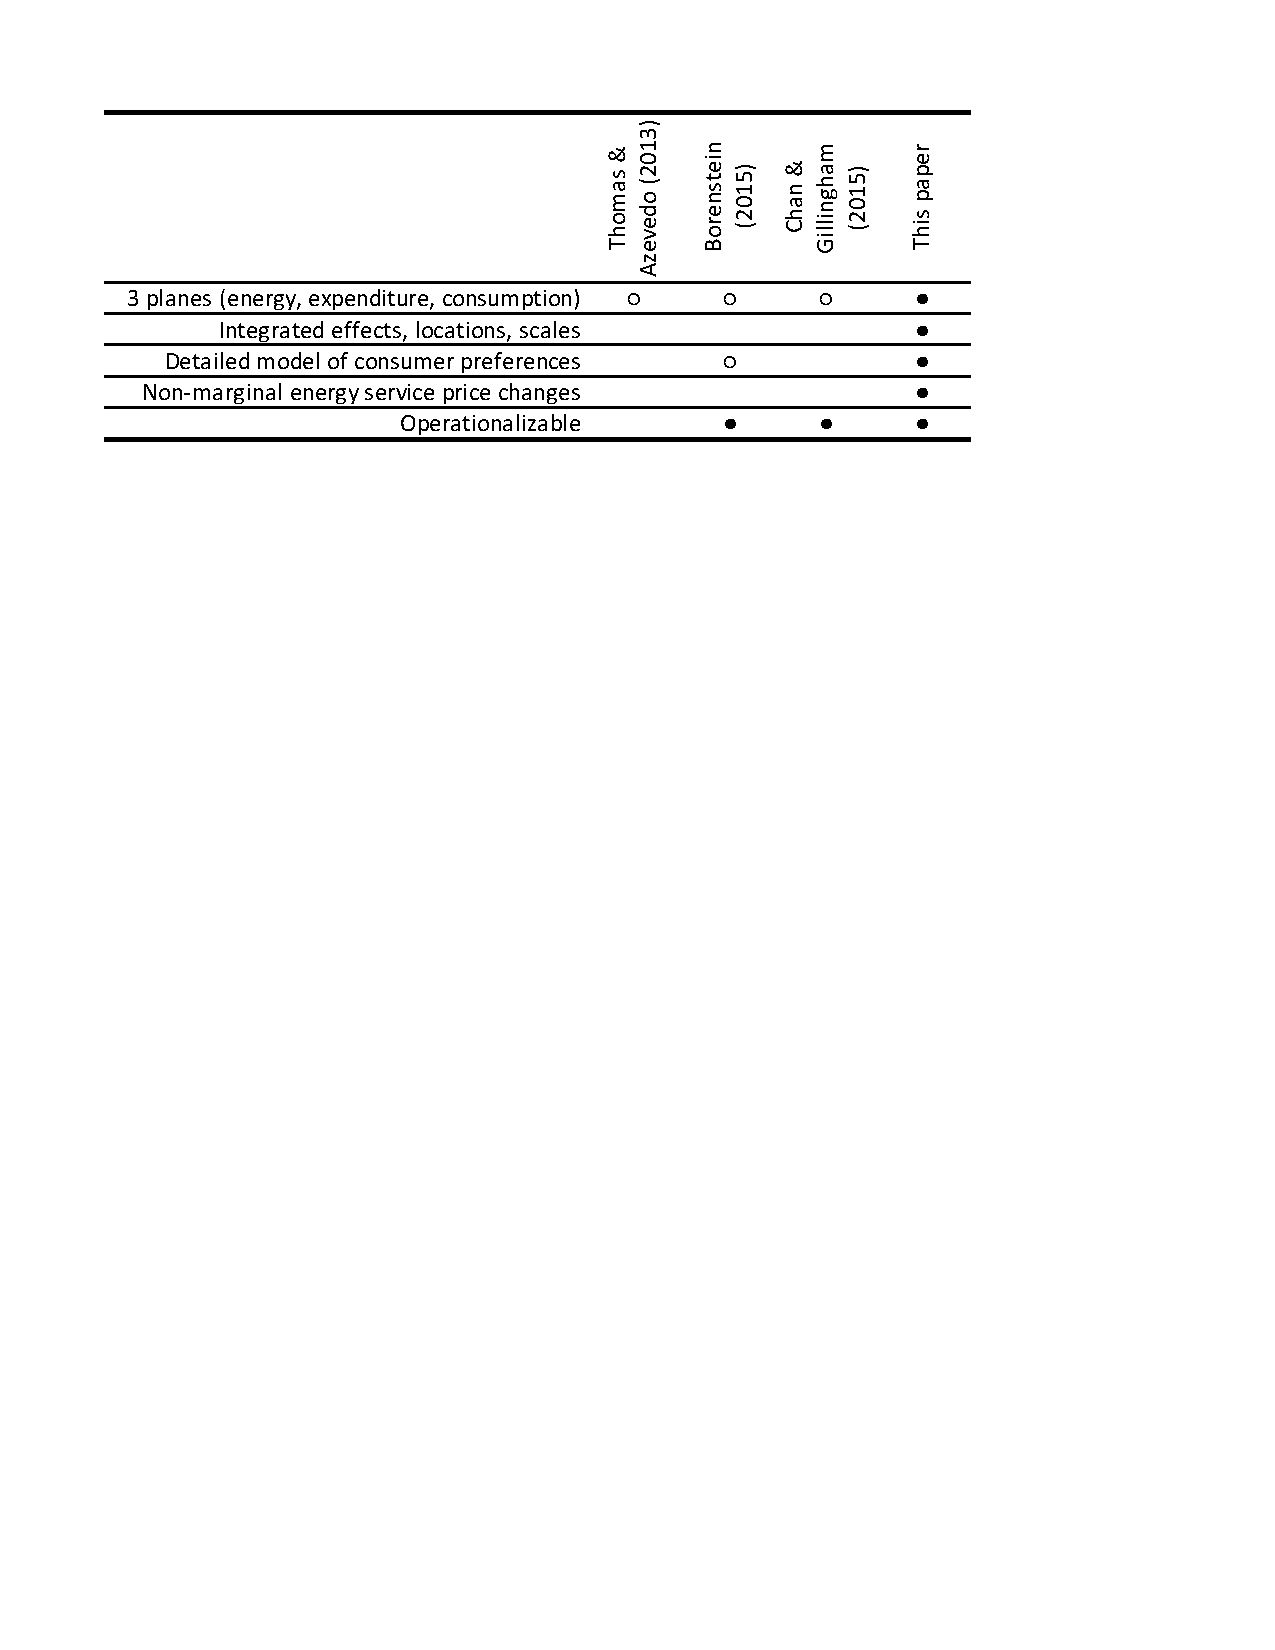
\includegraphics[width=1\linewidth]{figure_other/PreviousFrameworksTable.pdf}
%   \label{tab:previous_frameworks}
% \end{table}

